% =============================================================================
% Lecture 03: Exponential Smoothing
% BSAD 8310: Business Forecasting
% University of Nebraska at Omaha
% =============================================================================

\documentclass[aspectratio=169, 11pt]{beamer}

% =============================================================================
% header.tex — BSAD 8310: Business Forecasting
% University of Nebraska at Omaha
% Beamer theme: UNO-branded, clean, professional
% =============================================================================

% ----------------------------- BEAMER THEME ----------------------------------
\usetheme{default}
\useinnertheme{rectangles}

% ----------------------------- UNO COLOR PALETTE -----------------------------
\definecolor{unoblue}{HTML}{005CA9}
\definecolor{unored}{HTML}{E41C38}
\definecolor{unogray}{HTML}{525252}
\definecolor{unogreen}{HTML}{15803d}
\definecolor{unolightblue}{HTML}{E8F0FA}
\definecolor{unolightred}{HTML}{FDECEA}
\definecolor{unolightgreen}{HTML}{F0FAF4}
\definecolor{unowhite}{HTML}{FFFFFF}

% Apply UNO colors to Beamer structure
\setbeamercolor{structure}{fg=unoblue}
\setbeamercolor{palette primary}{bg=unoblue, fg=white}
\setbeamercolor{palette secondary}{bg=unoblue!80!black, fg=white}
\setbeamercolor{palette tertiary}{bg=unoblue!60!black, fg=white}
\setbeamercolor{frametitle}{bg=unoblue, fg=white}
\setbeamercolor{frametitle right}{bg=unoblue!80!black}
\setbeamercolor{title}{fg=unoblue}
\setbeamercolor{subtitle}{fg=unogray}
\setbeamercolor{author in head/foot}{bg=unoblue, fg=white}
\setbeamercolor{title in head/foot}{bg=unoblue!80, fg=white}
\setbeamercolor{date in head/foot}{bg=unoblue!60, fg=white}
\setbeamercolor{page number in head/foot}{bg=unoblue!60, fg=white}
\setbeamercolor{block title}{bg=unoblue, fg=white}
\setbeamercolor{block body}{bg=unolightblue}
\setbeamercolor{block title alerted}{bg=unored, fg=white}
\setbeamercolor{block body alerted}{bg=unolightred}
\setbeamercolor{block title example}{bg=unogreen, fg=white}
\setbeamercolor{block body example}{bg=unolightgreen}
\setbeamercolor{itemize item}{fg=unoblue}
\setbeamercolor{itemize subitem}{fg=unored}
\setbeamercolor{enumerate item}{fg=unoblue}
\setbeamercolor{enumerate subitem}{fg=unored}
\setbeamercolor{alerted text}{fg=unored}

% ----------------------------- FONTS -----------------------------------------
\usefonttheme{professionalfonts}
\usefonttheme[onlymath]{serif}       % serif math; sans-serif text
\setbeamerfont{frametitle}{size=\large, series=\bfseries}
\setbeamerfont{title}{size=\LARGE, series=\bfseries}
\setbeamerfont{subtitle}{size=\large}
\setbeamerfont{block title}{size=\normalsize, series=\bfseries}
\setbeamerfont{footline}{size=\tiny}

% ----------------------------- LAYOUT ----------------------------------------
\setbeamersize{text margin left=0.5cm, text margin right=0.5cm}
\setbeamertemplate{navigation symbols}{}   % remove navigation buttons
\setbeamertemplate{itemize items}[circle]
\setbeamertemplate{enumerate items}[default]

% Custom footline: [Course] [Title] [Page/Total]
\setbeamertemplate{footline}{%
  \leavevmode%
  \hbox{%
    \begin{beamercolorbox}[wd=.33\paperwidth, ht=2.5ex, dp=1ex, left, leftskip=4pt]
      {author in head/foot}%
      \usebeamerfont{author in head/foot}\insertshortauthor
    \end{beamercolorbox}%
    \begin{beamercolorbox}[wd=.34\paperwidth, ht=2.5ex, dp=1ex, center]
      {title in head/foot}%
      \usebeamerfont{title in head/foot}\insertshorttitle
    \end{beamercolorbox}%
    \begin{beamercolorbox}[wd=.33\paperwidth, ht=2.5ex, dp=1ex, right, rightskip=4pt]
      {date in head/foot}%
      \usebeamerfont{date in head/foot}%
      \insertframenumber{} / \inserttotalframenumber
    \end{beamercolorbox}%
  }%
  \vskip0pt%
}

% Frametitle with thin accent line
\setbeamertemplate{frametitle}{%
  \vskip0.1cm
  \insertframetitle
  \vskip0.05cm
  \color{unored}\rule{\textwidth}{0.5pt}
}

% Title page
\setbeamertemplate{title page}{%
  \vfill
  \begin{center}
    {\color{unoblue}\rule{\textwidth}{2pt}}\\[0.3cm]
    {\usebeamerfont{title}\usebeamercolor[fg]{title}\inserttitle}\\[0.2cm]
    {\usebeamerfont{subtitle}\usebeamercolor[fg]{subtitle}\insertsubtitle}\\[0.3cm]
    {\color{unored}\rule{\textwidth}{0.5pt}}\\[0.4cm]
    {\small\insertauthor}\\[0.1cm]
    {\small\insertinstitute}\\[0.1cm]
    {\small\insertdate}
  \end{center}
  \vfill
}

% ----------------------------- PACKAGES --------------------------------------

% Math
\usepackage{amsmath}
\usepackage{amssymb}
\usepackage{mathtools}
\usepackage{bm}                    % bold math symbols

% Graphics & color
\usepackage{graphicx}
\usepackage{xcolor}
\usepackage{tikz}
\usetikzlibrary{arrows.meta, positioning, shapes, fit, backgrounds, calc}
\usepackage{pgfplots}
\pgfplotsset{compat=1.18}

% Tables
\usepackage{booktabs}
\usepackage{array}
\usepackage{multirow}
\usepackage{tabularx}

% Typography
\usepackage{microtype}
\usepackage{url}
\usepackage{hyperref}
\hypersetup{colorlinks=true, linkcolor=unoblue, urlcolor=unoblue, citecolor=unogray}

% Code listings (no shell-escape required)
\usepackage{listings}
\lstset{
  language=Python,
  basicstyle=\ttfamily\footnotesize,
  keywordstyle=\color{unoblue}\bfseries,
  stringstyle=\color{unogreen},
  commentstyle=\color{unogray}\itshape,
  numberstyle=\tiny\color{unogray},
  breaklines=true,
  showstringspaces=false,
  frame=single,
  rulecolor=\color{unogray!40},
  backgroundcolor=\color{unogray!5},
  xleftmargin=0.5em,
  xrightmargin=0.5em,
}

% Bibliography
\usepackage[backend=bibtex, style=authoryear, maxcitenames=2]{biblatex}
\addbibresource{../Bibliography_base.bib}

% Colored text helpers
\usepackage{tcolorbox}
\tcbuselibrary{skins, breakable, listingsutf8}

% ----------------------------- CUSTOM ENVIRONMENTS ---------------------------

% keybox: UNO-blue background — for key results, formulas, takeaways
\newtcolorbox{keybox}{
  enhanced,
  colback=unoblue,
  colframe=unoblue!80!black,
  coltitle=white,
  coltext=white,
  fonttitle=\bfseries,
  boxrule=0pt,
  arc=3pt,
  left=4pt, right=4pt, top=3pt, bottom=3pt,
}

% definitionbox: blue left-rule with title — for formal definitions
\newtcolorbox{definitionbox}[1]{
  enhanced,
  title={#1},
  colback=unolightblue,
  colframe=unoblue,
  coltitle=unoblue,
  fonttitle=\bfseries,
  boxrule=0pt,
  leftrule=3pt,
  arc=0pt,
  left=4pt, right=4pt, top=3pt, bottom=3pt,
}

% warningbox: red-accent — for pitfalls, assumption violations, common errors
\newtcolorbox{warningbox}{
  enhanced,
  colback=unolightred,
  colframe=unored,
  coltitle=white,
  fonttitle=\bfseries,
  boxrule=0pt,
  leftrule=3pt,
  arc=0pt,
  left=4pt, right=4pt, top=3pt, bottom=3pt,
}

% examplebox: green-accent with title — for worked examples, business applications
\newtcolorbox{examplebox}[1]{
  enhanced,
  title={#1},
  colback=unolightgreen,
  colframe=unogreen,
  coltitle=unogreen,
  fonttitle=\bfseries,
  boxrule=0pt,
  leftrule=3pt,
  arc=0pt,
  left=4pt, right=4pt, top=3pt, bottom=3pt,
}

% ----------------------------- MATH SHORTCUTS --------------------------------
\newcommand{\E}{\mathbb{E}}
\newcommand{\Var}{\operatorname{Var}}
\newcommand{\Cov}{\operatorname{Cov}}
\newcommand{\Corr}{\operatorname{Corr}}
\newcommand{\MSE}{\operatorname{MSE}}
\newcommand{\RMSE}{\operatorname{RMSE}}
\newcommand{\MAE}{\operatorname{MAE}}
\newcommand{\MASE}{\operatorname{MASE}}
\newcommand{\yhat}{\hat{y}}
\newcommand{\bhat}{\hat{\beta}}
\newcommand{\eps}{\varepsilon}
\newcommand{\given}{\,|\,}

% ----------------------------- SLIDE HELPERS ---------------------------------
% Section title slide (call at start of each section)
\newcommand{\sectionslide}[2]{%
  \begin{frame}
    \vfill
    \begin{center}
      {\color{unoblue}\rule{0.6\textwidth}{2pt}}\\[0.4cm]
      {\Large\bfseries\color{unoblue} #1}\\[0.2cm]
      {\normalsize\color{unogray} #2}\\[0.4cm]
      {\color{unored}\rule{0.6\textwidth}{1pt}}
    \end{center}
    \vfill
  \end{frame}
}

% Muted text
\newcommand{\muted}[1]{{\color{unogray}#1}}

% Key term
\newcommand{\key}[1]{{\color{unoblue}\textbf{#1}}}

% Positive / negative annotations
\newcommand{\pos}[1]{{\color{unogreen}#1}}
\newcommand{\negc}[1]{{\color{unored}#1}}


% ---- Lecture metadata --------------------------------------------------------
\title{Exponential Smoothing}
\subtitle{BSAD 8310: Business Forecasting --- Lecture 3}
\author{Department of Economics}
\institute{University of Nebraska at Omaha}
\date{Spring 2026}

% =============================================================================
\begin{document}
% =============================================================================

\begin{frame}
  \titlepage
\end{frame}

% --- Outline -----------------------------------------------------------------
\begin{frame}{Lecture 3: Outline}
  \tableofcontents
\end{frame}

% =============================================================================
\section{Motivation: Adaptive Averaging}
% =============================================================================

\sectionslide{Motivation: Adaptive Averaging}{%
  Regression treats all observations equally --- but recent observations carry more information.}

% --- Slide: The equal-weight problem ------------------------------------------
\begin{frame}{The Equal-Weight Problem}
  In OLS regression, \emph{every} observation receives equal implicit weight:
  \[
    \hat{\boldsymbol{\beta}} = (\mathbf{X}'\mathbf{X})^{-1}\mathbf{X}'\mathbf{y}
    \qquad \Rightarrow \qquad
    \hat{y}_{T+h|T} = \mathbf{x}_{T+h}'\hat{\boldsymbol{\beta}}
  \]
  \begin{warningbox}
    When the data-generating process \textbf{drifts over time} --- structural
    breaks, changing growth rates, evolving seasonality --- old observations
    \textbf{contaminate} the forecast.
  \end{warningbox}
  \begin{examplebox}{Business context}
    A retailer's sales pattern shifts after a store renovation.
    OLS keeps fitting to pre-renovation data, systematically over- or
    under-forecasting for months afterward.
  \end{examplebox}
\end{frame}

% --- Slide: Exponential weighting idea ----------------------------------------
\begin{frame}{The Exponential Weighting Idea}
  \textbf{Idea:} assign geometrically declining weights to past observations.
  \begin{center}
    \begin{tabular}{lcc}
      \toprule
      Observation & Age & Weight \\
      \midrule
      $y_T$     & 0 & $\alpha$ \\
      $y_{T-1}$ & 1 & $\alpha(1-\alpha)$ \\
      $y_{T-2}$ & 2 & $\alpha(1-\alpha)^2$ \\
      $y_{T-j}$ & $j$ & $\alpha(1-\alpha)^j$ \\
      \bottomrule
    \end{tabular}
  \end{center}
  Weights sum to 1: $\;\sum_{j=0}^{\infty}\alpha(1-\alpha)^j = 1$ for $0 < \alpha \leq 1$.
  \begin{keybox}
    A single parameter $\alpha$ controls how fast old observations are
    \textbf{forgotten}.
    \quad \textbf{$\alpha \approx 1$}: almost all weight on the latest value.
    \quad \textbf{$\alpha \approx 0$}: long memory.
  \end{keybox}
\end{frame}

% =============================================================================
\section{Simple Exponential Smoothing}
% =============================================================================

\sectionslide{Simple Exponential Smoothing}{%
  One parameter, one component: the level.}

% --- Slide: SES definition ----------------------------------------------------
\begin{frame}{Simple Exponential Smoothing (SES)}
  \begin{definitionbox}{Simple Exponential Smoothing}
    {\small Let $\ell_t$ denote the \textbf{level} at time $t$. SES updates:
    \[
      \ell_t \;=\; \alpha\, y_t \;+\; (1-\alpha)\,\ell_{t-1},
      \qquad 0 < \alpha \leq 1
    \]
    with initialization $\ell_0$ estimated from the data.}
  \end{definitionbox}
  \vspace{0.1cm}
  \textbf{Recursive expansion} reveals the exponential weights:
  \[
    \ell_t \;=\; \alpha\sum_{j=0}^{t-1}(1-\alpha)^j\,y_{t-j}
              \;+\; (1-\alpha)^t\,\ell_0
  \]
  \muted{\footnotesize\itshape
    As $t \to \infty$, the initialization term $(1-\alpha)^t\ell_0 \to 0$
    for any $\alpha > 0$ --- the starting value eventually becomes irrelevant.}
\end{frame}

% --- Slide: Error-correction form ---------------------------------------------
\begin{frame}{The Error-Correction Form}
  SES can be rewritten as an \textbf{error-correction equation}:
  \[
    \ell_t \;=\; \ell_{t-1} \;+\; \alpha\underbrace{(y_t - \ell_{t-1})}_{e_t}
           \;=\; \ell_{t-1} + \alpha\,e_t
  \]
  where $e_t = y_t - \ell_{t-1}$ is the one-step-ahead forecast error.
  \muted{\footnotesize\itshape (SES is equivalent to ARIMA(0,1,1) --- see Lecture 4.)}
  \begin{keybox}
    At each period the level is \textbf{updated in proportion to the latest
    error}. $\alpha$ controls the speed of adaptation.
  \end{keybox}
  \begin{columns}[T]
    \column{0.48\textwidth}
      \textbf{Large $\alpha$ (e.g.\ 0.8):}
      \begin{itemize}\small
        \item Reacts quickly to shocks
        \item Noisy, volatile forecasts
        \item Good for rapidly changing series
      \end{itemize}
    \column{0.48\textwidth}
      \textbf{Small $\alpha$ (e.g.\ 0.1):}
      \begin{itemize}\small
        \item Slow adaptation
        \item Smooth, stable forecasts
        \item Good for slowly evolving, near-stationary series
      \end{itemize}
  \end{columns}
\end{frame}

% --- Slide: Estimating alpha + SES forecast -----------------------------------
\begin{frame}{Estimating $\alpha$ and the SES Forecast}
  \textbf{Parameter estimation:} choose $\alpha$ and $\ell_0$ to minimize
  the sum of squared one-step-ahead errors \parencite[][Ch.~8]{Hyndman2021}:
  \[
    \min_{\alpha,\,\ell_0}\;\sum_{t=1}^{T}(y_t - \ell_{t-1})^2,
    \qquad 0 < \alpha \leq 1
  \]
  Solved numerically (bounded nonlinear optimization).

  \vspace{0.15cm}
  \textbf{Forecast:} for \emph{any} horizon $h \geq 1$,
  \[
    \hat{y}_{T+h|T} \;=\; \ell_T
  \]
  \begin{warningbox}
    SES produces a \textbf{flat forecast} --- the same value at all horizons.
    Appropriate only when the series has \emph{no trend and no seasonality}.
  \end{warningbox}
  \muted{\footnotesize\itshape
    Socratic: if $y_T = 110$, $\ell_{T-1} = 104$, and $\hat{\alpha} = 0.6$,
    what is $\hat{y}_{T+1|T}$?}
\end{frame}

% --- Slide: SES example + boundary cases --------------------------------------
\begin{frame}{SES in Context: Boundary Cases}
  \begin{examplebox}{US Retail Sales (RSXFS)}
    {\small Estimated $\hat{\alpha} \approx 0.70$ --- fast adaptation.
    Forecast for month $T{+}1$ equals the final smoothed level $\ell_T$.
    Lab 3 compares RMSE against Lecture 1--2 benchmarks.}
  \end{examplebox}
  \vspace{0.2cm}
  \textbf{Connection to benchmarks:}
  \begin{center}
    \begin{tabular}{ll}
      \toprule
      \textbf{Special case} & \textbf{Model} \\
      \midrule
      $\alpha = 1$ & Na\"{i}ve forecast: $\hat{y}_{T+h|T} = y_T$ \\
      $\alpha \to 0$ (large $T$) & Historical mean: $\hat{y}_{T+h|T} = \bar{y}$ \\
      \bottomrule
    \end{tabular}
  \end{center}
  \begin{keybox}
    SES \textbf{nests} both extreme benchmarks from Lecture 1.
    $\hat{\alpha}$ locates the optimal point between ``forget everything''
    and ``forget nothing.''
  \end{keybox}
\end{frame}

% =============================================================================
\section{Holt's Linear Method}
% =============================================================================

\sectionslide{Holt's Linear Method}{%
  Add a second component for trend: level and slope updated separately.}

% --- Slide: Two components ----------------------------------------------------
\begin{frame}{Holt's Linear Method: Level and Trend}
  \begin{definitionbox}{Holt's Linear Exponential Smoothing}
    {\small
    \textbf{Level:}
    $\;\ell_t = \alpha\, y_t + (1-\alpha)\,(\ell_{t-1} + b_{t-1})$\\[4pt]
    \textbf{Trend:}
    $\;b_t = \beta^*(\ell_t - \ell_{t-1}) + (1-\beta^*)\,b_{t-1}$\\[4pt]
    Parameters: $\;0 < \alpha \leq 1$, $\;0 < \beta^* \leq 1$
    \hfill\muted{\footnotesize\parencite{Holt2004}}
    }
  \end{definitionbox}
  \vspace{0.1cm}
  \begin{columns}[T]
    \column{0.52\textwidth}
      \textbf{Interpretation:}
      \begin{itemize}
        \item $\ell_t$: where the series is \emph{now}
        \item $b_t$: the current growth rate
        \item $\beta^*$ controls how fast the slope adapts
      \end{itemize}
    \column{0.44\textwidth}
      \textbf{$h$-step forecast:}
      \[
        \hat{y}_{T+h|T} = \ell_T + h\,b_T
      \]
      Extrapolates the current trend linearly.
  \end{columns}
  \muted{\footnotesize\itshape
    SES is nested inside Holt: take $\beta^* \to 0$ and $b_0 = 0$ (so $b_t = 0$ for all $t$).}
\end{frame}

% --- Slide: Damped trend ------------------------------------------------------
\begin{frame}{The Damped Trend}
  Linear extrapolation can be \negc{unrealistic} for long horizons ---
  trends rarely persist indefinitely.
  \begin{columns}[T]
    \column{0.50\textwidth}
      \textbf{Damped-trend modification \parencite{Gardner2006}:}
      \[
        \hat{y}_{T+h|T} = \ell_T + \!\sum_{j=1}^{h}\phi^j b_T,
        \quad 0 < \phi < 1
      \]
      \begin{keybox}
        {\small
        $\phi \to 1$: standard Holt (no damping).\\
        $\phi \to 0$: forecast $\to \ell_T$ (flat; trend vanishes).\\
        \textbf{Use damped by default for $h > 6$.}
        }
      \end{keybox}
    \column{0.47\textwidth}
      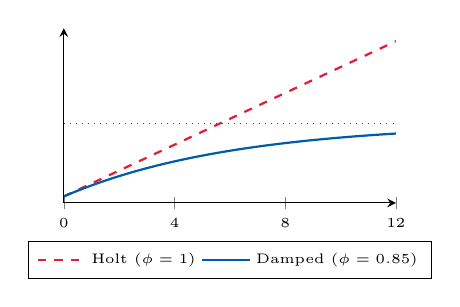
\begin{tikzpicture}
        \begin{axis}[
          width=5.8cm, height=3.8cm,
          xlabel={\small Horizon $h$},
          xmin=0, xmax=12, ymin=98, ymax=152,
          xtick={0,4,8,12}, ytick=\empty,
          axis lines=left,
          tick label style={font=\tiny},
          label style={font=\small},
          legend style={font=\tiny, at={(0.5,-0.22)}, anchor=north,
                        legend columns=2},
        ]
          % Linear: 100 + 4h
          \addplot[color=unored, thick, dashed, domain=0:12, samples=25]
            {100 + 4*x};
          \addlegendentry{Holt ($\phi=1$)}
          % Damped: 100 + 4*phi*(1-phi^h)/(1-phi), phi=0.85
          \addplot[color=unoblue, thick, domain=0:12, samples=50]
            {100 + 4*0.85*(1-0.85^x)/(0.15)};
          \addlegendentry{Damped ($\phi=0.85$)}
          % Asymptote at 100 + 4*0.85/0.15 = 122.67
          \addplot[color=unoblue, very thin, dotted, domain=0:12] {122.67};
        \end{axis}
      \end{tikzpicture}
  \end{columns}
  \muted{\footnotesize\itshape
    Socratic: with $\ell_T = 100$, $b_T = 4$, $\phi = 0.85$,
    what is $\hat{y}_{T+3|T}$? (Hint: compute $\phi + \phi^2 + \phi^3$.) \quad
    Why might large $\beta^*$ cause erratic forecasts when spikes occur?}
\end{frame}

% =============================================================================
\section{Holt-Winters Seasonal Method}
% =============================================================================

\sectionslide{Holt-Winters Seasonal Method}{%
  Add a third component for seasonality: level, trend, and season.}

% --- Slide: Three-component model + additive equations ------------------------
\begin{frame}{Three-Component Decomposition}
  The \textbf{additive Holt-Winters model} \parencite{Winters1960}:
  \[
    y_t \;=\; \ell_t \;+\; b_t \;+\; s_t \;+\; \varepsilon_t
  \]
  where $s_t$ is the seasonal component with period $m$.
  \begin{definitionbox}{Holt-Winters Additive Update Equations}
    {\small
    $\ell_t = \alpha(y_t - s_{t-m}) + (1-\alpha)(\ell_{t-1}+b_{t-1})$\\[3pt]
    $b_t = \beta^*(\ell_t - \ell_{t-1}) + (1-\beta^*)\,b_{t-1}$\\[3pt]
    $s_t = \gamma(y_t - \ell_{t-1} - b_{t-1}) + (1-\gamma)\,s_{t-m}$\\[3pt]
    Parameters: $0 < \alpha \leq 1$, $0 < \beta^* \leq 1$,
    $0 < \gamma \leq 1{-}\alpha$; seasonal period $m$
    }
  \end{definitionbox}
  \muted{\footnotesize\itshape
    The $m$ seasonal indices sum to zero over one full period.
    For monthly data, $m = 12$.}
\end{frame}

% --- Slide: Additive vs multiplicative ----------------------------------------
\begin{frame}{Additive vs.\ Multiplicative Seasonality}
  \begin{columns}[T]
    \column{0.48\textwidth}
      \textbf{Additive forecast:}
      \[
        \hat{y}_{T+h|T} = \ell_T + h\,b_T + s_{T+h-m}
      \]
    \column{0.48\textwidth}
      \textbf{Multiplicative forecast:}
      \[
        \hat{y}_{T+h|T} = (\ell_T + h\,b_T)\,s_{T+h-m}
      \]
  \end{columns}
  \begin{center}
    {\small
    \begin{tabular}{lll}
      \toprule
      \textbf{Variant} & \textbf{Seasonal component} & \textbf{When to use} \\
      \midrule
      Additive  & $\ell_t + s_t$ & Seasonal amplitude \emph{constant} in size \\
      Multiplicative & $\ell_t \times s_t$ & Seasonal amplitude \emph{proportional} to level \\
      \bottomrule
    \end{tabular}
    }
  \end{center}
  \begin{examplebox}{US Retail Sales (RSXFS)}
    {\small The holiday-season spike grows as overall sales grow
    $\Rightarrow$ \textbf{multiplicative seasonality} is usually preferred.}
  \end{examplebox}
\end{frame}

% --- Slide: Estimation and initialization ------------------------------------
\begin{frame}{Estimation and Initialization}
  \textbf{Parameters to estimate:} $\alpha$, $\beta^*$, $\gamma$, plus initial
  values $\ell_0$, $b_0$, and $m$ seasonal indices $s_{1-m}, \ldots, s_0$.

  \textbf{Initialization strategies:}
  \begin{itemize}\small
    \item \textbf{Classical:} first-season average for $\ell_0$;
          first-to-second-season slope for $b_0$;
          seasonal differences for $s_1, \ldots, s_m$
    \item \textbf{Optimized:} jointly minimize SSE over all parameters
          \emph{and} initial values (default in \texttt{statsmodels})
  \end{itemize}
  \begin{warningbox}
    Holt-Winters requires at least $\mathbf{2m}$ observations to initialize.
    With $m = 12$, you need $\geq 24$ months of data.
  \end{warningbox}
  \muted{\footnotesize\itshape
    Socratic: if the December spike triples over ten years, which variant
    is appropriate and what does that imply for $\hat{\gamma}$?}
\end{frame}

% =============================================================================
\section{The ETS Framework}
% =============================================================================

\sectionslide{The ETS Framework}{%
  A unified state space taxonomy: Error $\times$ Trend $\times$ Seasonal.}

% --- Slide: ETS taxonomy ------------------------------------------------------
\begin{frame}{ETS: Error $\times$ Trend $\times$ Seasonal}
  \textcite{Hyndman2021} unify all exponential smoothing variants as
  \textbf{state space models} with a single error source.
  \begin{center}
    {\small
    \begin{tabular}{lll}
      \toprule
      \textbf{Component} & \textbf{Options} & \textbf{Meaning} \\
      \midrule
      Error ($E$)    & A, M
                     & Additive / Multiplicative \\
      Trend ($T$)    & N, A, A\textsubscript{d}
                     & None / Additive / Additive damped \\
      Seasonal ($S$) & N, A, M
                     & None / Additive / Multiplicative \\
      \bottomrule
    \end{tabular}
    }
  \end{center}
  $2 \times 3 \times 3 = 18$ combinations; some are inadmissible,
  giving \textbf{15 valid ETS models}.

  \vspace{0.1cm}
  \begin{columns}[T]
    \column{0.48\textwidth}
      \textbf{ETS(A,N,N)} $=$ SES\\
      \textbf{ETS(A,A,N)} $=$ Holt linear\\
      \textbf{ETS(A,A\textsubscript{d},N)} $=$ Holt damped
    \column{0.48\textwidth}
      \textbf{ETS(A,A,A)} $=$ Holt-Winters additive\\
      \textbf{ETS(A,A,M)} $=$ Holt-Winters multiplicative\\
      \muted{\small (and 10 more variants)}
  \end{columns}
\end{frame}

% --- Slide: State space representation ----------------------------------------
\begin{frame}{State Space Representation}
  Every ETS model can be written as a \textbf{state space model} (additive-error form shown):
  \[
    y_t = h(\mathbf{x}_{t-1}) + k(\mathbf{x}_{t-1})\,\varepsilon_t,
    \qquad \varepsilon_t \overset{\mathrm{iid}}{\sim} \mathcal{N}(0,\sigma^2)
  \]
  \[
    \mathbf{x}_t = f(\mathbf{x}_{t-1}) + g(\mathbf{x}_{t-1})\,\varepsilon_t
  \]
  where $\mathbf{x}_t = (\ell_t,\, b_t,\, s_t, \ldots)'$ is the state vector.

  \vspace{0.1cm}
  \begin{columns}[T]
    \column{0.50\textwidth}
      \textbf{Additive error} (\texttt{E = A}):
      \begin{itemize}\small
        \item Gaussian likelihood, closed-form
              prediction interval (PI)
        \item Easier to interpret
      \end{itemize}
    \column{0.46\textwidth}
      \textbf{Multiplicative error} (\texttt{E = M}):
      \begin{itemize}\small
        \item Often better RMSE
        \item \negc{No closed-form PI}
      \end{itemize}
  \end{columns}
  \begin{keybox}
    The state space form enables \textbf{maximum likelihood estimation}
    and principled prediction intervals.
  \end{keybox}
  \muted{\footnotesize\itshape
    Notation: $\varepsilon_t$ here is the model innovation.
    For additive-error models, $\varepsilon_t \equiv e_t$ (forecast error);
    for multiplicative-error models, $\varepsilon_t = e_t / \ell_{t-1}$.}
\end{frame}

% --- Slide: Automatic model selection -----------------------------------------
\begin{frame}{Automatic Model Selection via AIC}
  Fit all 15 valid ETS models; select by minimum AIC.
  \parencite[][Ch.~8]{Hyndman2021}:
  \[
    \mathrm{AIC} = -2\hat{L} + 2p,
    \qquad \hat{L} = \text{maximized log-likelihood}
  \]
  \begin{center}
    {\small
    \begin{tabular}{lll}
      \toprule
      \textbf{ETS model} & \textbf{Key features} & \textbf{Typical application} \\
      \midrule
      ETS(A,N,N) & No trend, no seasonal   & Stable, level series \\
      ETS(A,A\textsubscript{d},N) & Damped trend & Long-horizon trending \\
      ETS(A,A,M) & Linear trend, mult.\ seasonal & Retail, tourism \\
      \bottomrule
    \end{tabular}
    }
  \end{center}
  \begin{keybox}
    In the M4 Competition, ETS-family methods ranked among the most
    accurate purely statistical approaches \parencite{Makridakis2020}.
  \end{keybox}
  \muted{\footnotesize\itshape
    Lab 3 uses \texttt{statsmodels.tsa.exponential\_smoothing.ets.ETSModel}
    for full AIC-based model selection across all valid ETS variants.}
\end{frame}

% =============================================================================
\section{Key Takeaways and Roadmap}
% =============================================================================

\sectionslide{Key Takeaways and Roadmap}{%
  ETS unifies exponential smoothing as state space models with AIC selection.}

% --- Slide: Key Takeaways -----------------------------------------------------
\begin{frame}{Key Takeaways}
  \begin{keybox}
    {\small
    \setlength{\itemsep}{1pt}
    \begin{enumerate}
      \item \textbf{Exponential weighting} gives more importance to recent
            observations; $\alpha$ controls the forgetting rate.
      \item \textbf{SES}: one smoothing parameter ($\alpha$), flat forecast ---
            nests na\"{i}ve ($\alpha{=}1$) and mean ($\alpha{\to}0$).
      \item \textbf{Holt}: adds trend component $b_t$ ---
            use the \emph{damped} variant for horizons $h > 6$.
      \item \textbf{Holt-Winters}: adds seasonal component $s_t$ ---
            choose additive vs.\ multiplicative based on whether
            amplitude scales with the level.
      \item \textbf{ETS framework}: unifies all methods as state space models;
            AIC selects the best variant automatically.
    \end{enumerate}
    }
  \end{keybox}
  \muted{\footnotesize\itshape
    All ETS models share the error-correction intuition: update each component
    in proportion to the latest forecast error.}
\end{frame}

% --- Slide: What's Next -------------------------------------------------------
\begin{frame}{What's Next: Stationarity and ARIMA}
  Exponential smoothing captures \textbf{level, trend, and seasonality}
  through adaptive updating.

  \vspace{0.15cm}
  \textbf{What ETS cannot easily handle:}
  \begin{itemize}\small
    \item Rich autocorrelation structure beyond a single AR(1)-like decay
    \item Integration and differencing in a principled statistical framework
    \item Combining external regressors with adaptive dynamics (ARIMAX)
  \end{itemize}
  \vspace{0.15cm}
  \begin{keybox}
    \textbf{Lecture 4:} Stationarity, differencing, and the ARIMA model
    family --- a regression-based approach to capturing autocorrelation.
  \end{keybox}
  \begin{center}
    \muted{\small
    \textbf{Lab 3:} Fit SES, Holt, Holt-Winters, and auto-ETS to RSXFS;
    compare RMSE / MAE with Lecture 1--2 benchmarks.
    }
  \end{center}
\end{frame}

% --- References ---------------------------------------------------------------
\begin{frame}[allowframebreaks]{References}
  \printbibliography[heading=none]
\end{frame}

\end{document}
